\documentclass{beamer}

\usepackage{amsthm, amsfonts, amsmath, amssymb} % Pacote para a definicao dos ambientes matematicos
\usepackage[brazilian]{babel}
\usepackage[utf8]{inputenc}
\usepackage[mathscr]{eucal}
\usepackage{tikz}
\usetikzlibrary{quotes, angles, intersections}
\newcommand{\R}{\mathbb{R}}
\newcommand{\D}{\mathscr{D}}
\newcommand{\Pp}{\mathscr{P}}
\newcommand{\Cc}{\mathscr{C}}
\newcommand{\E}{\mathscr{E}}
\newcommand{\norm}[2][2]{\left\lVert#2\right\rVert_{#1}}

\author{Danilo Tedeschi\\Dra. Marina Andretta}
\title{Fixed-Shape Ellipse by Three Points}
\institute{Universidade de São Paulo}
\date{25 de Outubro de 2019}

\begin{document}
	
	\begin{frame}[t,plain]
		\titlepage
	\end{frame}
	
	\begin{frame}{Introduction}
		The shape of an ellipse is given by its major-axis and minor-axis, $(a, b) \in \mathbb{R}^2$, with $a > b > 0$.
		
		\begin{figure}[H]
			\centering
			
			%\caption{The ellipse as a parametric curve.}
			

%\tikzset{every picture/.style={line width=0.75pt}} %set default line width to 0.75pt        

\begin{tikzpicture}[x=0.75pt,y=0.75pt,yscale=-1,xscale=1]
%uncomment if require: \path (0,300); %set diagram left start at 0, and has height of 300

%Shape: Ellipse [id:dp1559950964552308] 
\draw   (100,180) .. controls (100,147.42) and (161.34,121) .. (237,121) .. controls (312.66,121) and (374,147.42) .. (374,180) .. controls (374,212.58) and (312.66,239) .. (237,239) .. controls (161.34,239) and (100,212.58) .. (100,180) -- cycle ;
%Straight Lines [id:da3716259356733107] 
\draw    (100,180) -- (374,180) ;


%Straight Lines [id:da9880464900454329] 
\draw    (237,121) -- (237,239) ;


%Shape: Brace [id:dp3973633345998604] 
\draw   (242,182) .. controls (242,186.67) and (244.33,189) .. (249,189) -- (293.5,189) .. controls (300.17,189) and (303.5,191.33) .. (303.5,196) .. controls (303.5,191.33) and (306.83,189) .. (313.5,189)(310.5,189) -- (358,189) .. controls (362.67,189) and (365,186.67) .. (365,182) ;
%Shape: Brace [id:dp94498526835576] 
\draw   (232,129) .. controls (227.34,128.79) and (224.9,131.01) .. (224.68,135.67) -- (224.47,140.23) .. controls (224.16,146.89) and (221.68,150.11) .. (217.01,149.9) .. controls (221.68,150.11) and (223.85,153.55) .. (223.54,160.21)(223.68,157.21) -- (223.33,164.68) .. controls (223.12,169.35) and (225.34,171.79) .. (230,172) ;

%Shape: Circle [id:dp8908034615999807] 




% Text Node
\draw (304,205) node   {$a$};
% Text Node
\draw (207,148.33) node   {$b$};
% Text Node



\end{tikzpicture}

			\label{fig:ellipse_params}
			\caption{An ellipse with shape parameters $a$ and $b$.}
		\end{figure}
		
	\end{frame}

\begin{frame}{Introduction}
	Here, the shape will be fixed and the center and angle of rotation are free.
	
	\begin{figure}
	\centering
	
	%\caption{The ellipse as a parametric curve.}
	\includegraphics[scale=.5]{3ellipses.pdf}
	\label{fig:ell}
	\caption{A fix-shape ellipse at different centers and with different angles of rotation.}
	\end{figure}
\end{frame}

\begin{frame}{Introduction}{Problem definition}
Given three points $u, v, w \in \R^2$, and the shape $(a,b) \in \R^2$ of an ellipse:
	\begin{figure}
	\centering
	
	%\caption{The ellipse as a parametric curve.}
	\includegraphics[scale=.5]{e3psol1.pdf}
	\label{fig:e3psol1}
	\caption{An instance of the problem.}
\end{figure}
\end{frame}

\begin{frame}{Introduction}{Problem definition}
	A solution is given by the ellipse's center $q \in \R^2$ and the angle of rotation $\theta \in [0, \pi)$, such that $u, v, w$ lie on its border. \textbf{We want to find every solution!}
	\begin{figure}
		\centering
		
		%\caption{The ellipse as a parametric curve.}
		\includegraphics[scale=.5]{e3psol2.pdf}
		\label{fig:e3psol2}
		\caption{Every solution for that instance.}
	\end{figure}
\end{frame}

\begin{frame}{Introduction}
	The equation of an ellipse is given by:
	
	\begin{equation*}
	\frac{\left(\left[\begin{array}{c}
	x-q_x\\
	y-q_y
		\end{array}\right]^T
		\left[\begin{array}{c}
		\cos\theta\\
		\sin\theta
		\end{array}\right]
		\right)^2}{a^2}+\frac{\left(\left[\begin{array}{c}
		x-q_x\\
		q_y-y
		\end{array}\right]^T
		\left[\begin{array}{c}
		\sin\theta\\
		\cos\theta
		\end{array}\right]
		\right)^2}{b^2} = 1.
	\end{equation*}
	
	\begin{itemize}
		\item Fixing the points $u, v, w$, we get $3$ equations and $3$ unknowns $(q_x, q_y, \theta)$.
		\item Finding every solution is difficult.
	\end{itemize}
\end{frame}

\begin{frame}{Transforming the problem}
	Let's make the problem simpler by transforming it into a circle problem.
	
	Given any non-colinear points, there is an unique circumscribed circle. Also, we can turn an axis-parallel ellipse into a circle:
	\begin{figure}
		\centering
		
		%\caption{The ellipse as a parametric curve.}
		\includegraphics[scale=.5]{el1.pdf}
		\label{fig:el1}
		\caption{Turning an ellipse with shape $(a, b)$ into a circle of radius $b$.}
	\end{figure}
	
\end{frame}

\begin{frame}{Transforming the problem}
	
	Let's rotate the points instead of rotating the ellipse. A solution can be transformed into the original problem.
	
	\begin{figure}
		\centering
		%\caption{Transforming an ellipse into a circle. T1, T2, and T3 represent the steps of the transformation.}
		\includegraphics{circumscribed-circle}
		\caption{}
		\label{fig:circumscribed-circle}
	\end{figure}
\end{frame}

\begin{frame}{Transforming the problem}
	Transforming it into a circle problem.
	
	\begin{itemize}
		\item Translate the points so $u=(0, 0)$.
		\item The ellipse is fixed, the points rotate.
		\item Scale the $x$-axis by $\frac{b}{a}$.
	\end{itemize}

	After the transformation, the points are defined by $\varphi(u, \theta), \varphi(v, \theta), \varphi(w, \theta)$:
	
	\begin{equation*}\label{eq:trpnts}
	\varphi(p, \theta)=\left[\begin{array}{cc}
	\frac{b}{a}&0\\
	0&1
	\end{array}\right]
	\left[\begin{array}{cc}
	\cos{\theta}&\sin{\theta}\\
	-\sin{\theta}&\cos{\theta}
	\end{array}\right]\left[\begin{array}{c}
	p_x\\
	p_y
	\end{array}\right].
	\end{equation*}
\end{frame}
	
\begin{frame}{Transforming the problem}
	Find every $\theta \in [0, \pi)$, such that:
	
	\begin{itemize}
		\item The circumscribe circle determined by: $\varphi(u, \theta), \varphi(v, \theta), \varphi(w, \theta)$ has radius $b$.
		
		\item As long as they are not colinear, there is an unique circumscribe circle by three points.
		
	\end{itemize}

	

\end{frame}

\begin{frame}{Fixed-shape ellipse by three points}
	There is a known formula for the radius of a circumscribed circle:

	\begin{equation*}
	R = \dfrac{\norm{\varphi(v, \theta)}\norm{\varphi(w, \theta)}\norm{\varphi(v, \theta)-\varphi(w, \theta)}   }{4A(\theta)}
	\end{equation*}
	
	\begin{itemize}
		\item $R$ is the radius.
		\item $A(\theta)$ is the area of the triangle defined by the points $\varphi(u, \theta), \varphi(v, \theta), \varphi(w, \theta)$.
	\end{itemize}
	\vspace{\baselineskip}
	

												
\end{frame}

\begin{frame}{Fixed-shape ellipse by three points}
We define the function $\xi : [0, \pi) \mapsto \R$:

	\begin{equation*}
	\xi(\theta) = 16b^2A(\theta)^2 - \norm{\varphi(v, \theta)}^2\norm{\varphi(w, \theta)}^2\norm{\varphi(v, \theta)-\varphi(w, \theta)}^2
	\end{equation*}
	
The roots of $\xi$ are solutions of our problem.
	\begin{figure}
	\centering

	%\caption{Transforming an ellipse into a circle. T1, T2, and T3 represent the steps of the transformation.}
	\includegraphics[scale=.5]{036}
	
%	\label{fig:circumscribed-circle}
\end{figure}
\end{frame}
	
\end{document}